\documentclass[12pt]{article}
 
\usepackage[margin=1in]{geometry}
\usepackage{amsmath,amsthm,amssymb}
\usepackage{mathtools}
\DeclarePairedDelimiter{\ceil}{\lceil}{\rceil}
%\usepackage{mathptmx}
\usepackage{accents}
\usepackage{comment}
\usepackage{graphicx}
\usepackage{IEEEtrantools}
 \usepackage{float}
 
\newcommand{\N}{\mathbb{N}}
\newcommand{\Z}{\mathbb{Z}}
\newcommand{\R}{\mathbb{R}}
\newcommand{\Q}{\mathbb{Q}}
\newcommand*\conj[1]{\bar{#1}}
\newcommand*\mean[1]{\bar{#1}}
\newcommand\widebar[1]{\mathop{\overline{#1}}}


\newcommand{\cc}{{\mathbb C}}
\newcommand{\rr}{{\mathbb R}}
\newcommand{\qq}{{\mathbb Q}}
\newcommand{\nn}{\mathbb N}
\newcommand{\zz}{\mathbb Z}
\newcommand{\aaa}{{\mathcal A}}
\newcommand{\bbb}{{\mathcal B}}
\newcommand{\rrr}{{\mathcal R}}
\newcommand{\fff}{{\mathcal F}}
\newcommand{\ppp}{{\mathcal P}}
\newcommand{\eps}{\varepsilon}
\newcommand{\vv}{{\mathbf v}}
\newcommand{\ww}{{\mathbf w}}
\newcommand{\xx}{{\mathbf x}}
\newcommand{\ds}{\displaystyle}
\newcommand{\Om}{\Omega}
\newcommand{\dd}{\mathop{}\,\mathrm{d}}
\newcommand{\ud}{\, \mathrm{d}}
\newcommand{\seq}[1]{\left\{#1\right\}_{n=1}^\infty}
\newcommand{\isp}[1]{\quad\text{#1}\quad}
\newcommand*\diff{\mathop{}\!\mathrm{d}}

\DeclareMathOperator{\imag}{Im}
\DeclareMathOperator{\re}{Re}
\DeclareMathOperator{\diam}{diam}
\DeclareMathOperator{\Tr}{Tr}
\DeclareMathOperator{\cis}{cis}

\def\upint{\mathchoice%
    {\mkern13mu\overline{\vphantom{\intop}\mkern7mu}\mkern-20mu}%
    {\mkern7mu\overline{\vphantom{\intop}\mkern7mu}\mkern-14mu}%
    {\mkern7mu\overline{\vphantom{\intop}\mkern7mu}\mkern-14mu}%
    {\mkern7mu\overline{\vphantom{\intop}\mkern7mu}\mkern-14mu}%
  \int}
\def\lowint{\mkern3mu\underline{\vphantom{\intop}\mkern7mu}\mkern-10mu\int}




\newenvironment{theorem}[2][Theorem]{\begin{trivlist}
\item[\hskip \labelsep {\bfseries #1}\hskip \labelsep {\bfseries #2.}]}{\end{trivlist}}
\newenvironment{lemma}[2][Lemma]{\begin{trivlist}
\item[\hskip \labelsep {\bfseries #1}\hskip \labelsep {\bfseries #2.}]}{\end{trivlist}}
\newenvironment{exercise}[2][Exercise]{\begin{trivlist}
\item[\hskip \labelsep {\bfseries #1}\hskip \labelsep {\bfseries #2.}]}{\end{trivlist}}
\newenvironment{problem}[2][Problem]{\begin{trivlist}
\item[\hskip \labelsep {\bfseries #1}\hskip \labelsep {\bfseries #2.}]}{\end{trivlist}}
\newenvironment{question}[2][Question]{\begin{trivlist}
\item[\hskip \labelsep {\bfseries #1}\hskip \labelsep {\bfseries #2.}]}{\end{trivlist}}
\newenvironment{corollary}[2][Corollary]{\begin{trivlist}
\item[\hskip \labelsep {\bfseries #1}\hskip \labelsep {\bfseries #2.}]}{\end{trivlist}}

\newenvironment{solution}{\begin{proof}[Solution]}{\end{proof}}
 
\begin{document}
 
% --------------------------------------------------------------
%                         Start here
% --------------------------------------------------------------
\title{Math 132A Homework 3}
\author{Ethan Martirosyan}
\date{\today}
\maketitle
\hbadness=99999
\hfuzz=50pt
\section*{Problem 1}
First, we write the Taylor polynomial as follows:
\[
f(x_0 + p) \approx f(x_0) + p^T \nabla f(x_0) + \frac{1}{2} p^T \nabla^2 f(x_0) p
\] Now, we note that
\begin{align*}
f(x_0) &= f(1,-1) = 3(1)^4 - 2(1)^3(-1)-4(1)^2(-1)^2 + 10(1)(-1)^3 + 2(-1)^4\\
&= 3 + 2 - 4 - 10 + 2 = -7
\end{align*}
Next, we compute
\[
\nabla f(x) = 
\begin{bmatrix}
12x_1^3 - 6x_1^2x_2 - 8x_1x_2^2 + 10x_2^3\\
-2x_1^3 - 8x_1^2x_2 + 30x_1x_2^2 + 8x_2^3
\end{bmatrix}
\] Now, we plug in the point $x_0 = (1,-1)$ to obtain
\[
\nabla f(x_0) = 
\begin{bmatrix}
12(1)^3 - 6(1)^2(-1) - 8(1)(-1)^2 + 10(-1)^3\\
-2(1)^3 - 8(1)^2(-1) + 30(1)(-1)^2 + 8(-1)^3
\end{bmatrix}
=
\begin{bmatrix}
0\\
28
\end{bmatrix}
\] From this, we get
\[
p^T \nabla f(x_0) =
\begin{bmatrix}
p_1 & p_2
\end{bmatrix}
\begin{bmatrix}
0\\
28
\end{bmatrix} = 0p_1 + 28p_2 = 28p_2
\] Now, we find the Hessian:
\[
\nabla^2 f(x) =
\begin{bmatrix}
\frac{\partial^2 f}{\partial x_1^2} & \frac{\partial^2 f}{\partial x_1 \partial x_2}\\
\frac{\partial^2 f}{\partial x_2 \partial x_1} & \frac{\partial^2 f}{\partial x_2^2}
\end{bmatrix}
= \begin{bmatrix}
36x_1^2 -12x_1x_2 - 8x_2^2 & -6x_1^2 - 16x_1x_2 + 30x_2^2\\
-6x_1^2 - 16x_1x_2 + 30x_2^2 & -8x_1^2 + 60x_1x_2 + 24x_2^2
\end{bmatrix}
\] so we get
\[
\nabla^2 f(x_0) = 
\begin{bmatrix}
36(1)^2 -12(1)(-1) - 8(-1)^2 & -6(1)^2 - 16(1)(-1) + 30(-1)^2\\
-6(1)^2 - 16(1)(-1) + 30(-1)^2 & -8(1)^2 + 60(1)(-1) + 24(-1)^2
\end{bmatrix}
=
\begin{bmatrix}
40 & 40\\
40 & -44
\end{bmatrix}
\] Using this, we obtain
\begin{align*}
p^T \nabla^2 f(x_0) p &= 
\begin{bmatrix}
p_1 & p_2
\end{bmatrix}
\begin{bmatrix}
40 & 40\\
40 & -44
\end{bmatrix}
\begin{bmatrix}
p_1\\
p_2
\end{bmatrix}
=
\begin{bmatrix}
p_1 & p_2
\end{bmatrix}
\begin{bmatrix}
40p_1 + 40p_2\\
40p_1 - 44p_2
\end{bmatrix}
\\
&= 40p_1^2 + 40p_1p_2 + 40p_1p_2 - 44p_2^2 = 40p_1^2 + 80p_1p_2 - 44p_2^2
\end{align*} so that
\[
\frac{1}{2}p^T \nabla^2 f(x_0) p = 20p_1^2 + 40p_1p_2 - 22p_2^2
\] Putting it all together, we find that
\[
f(x_0) + p^T \nabla f(x_0) + \frac{1}{2} p^T \nabla^2 f(x_0) p = -7 + 28p_2 + 20p_1^2 + 40p_1p_2 - 22p_2^2
\] Now, we plug in $p = (0.1,0.01)$ to obtain
\[
f(x_0 + p) \approx  -7 + 28(0.01) + 20(0.1)^2 + 40(0.1)(0.01) - 22(0.01)^2 = -6.4822
\] An exact evaluation yields
\begin{align*}
f(x_0+p) &= f(1.1,-0.99) = 3(1.1)^4 - 2(1.1)^3(-0.99) - 4(1.1)^2(-0.99)^2+10(1.1)(-0.99)^3 + 2(-0.99)^4 \\
&= -6.4681
\end{align*} The difference between these two is
\[
\vert -6.4822 + 6.4681 \vert = 0.0141
\]
\newpage
\section*{Problem 2}
The first three terms of the Taylor series are
\[
f(x_0 + p) \approx f(x_0) + p^T \nabla f(x_0) + \frac{1}{2} p^T \nabla^2 f(x_0) p
\]
First, we find
\[
f(x_0) = f(3,4) = \sqrt{3^2+4^2} = \sqrt{9+16} = \sqrt{25} = 5
\] Next, we compute
\[
\nabla f(x) = 
\begin{bmatrix}
\frac{\partial}{\partial x_1} \sqrt{x_1^2 + x_2^2}\\
\frac{\partial}{\partial x_2} \sqrt{x_1^2+x_2^2}
\end{bmatrix}
=
\begin{bmatrix}
\frac{x_1}{\sqrt{x_1^2+x_2^2}}\\
\frac{x_2}{\sqrt{x_1^2+x_2^2}}
\end{bmatrix}
\] so that
\[
\nabla f(x_0) =
\begin{bmatrix}
3/5\\
4/5
\end{bmatrix}
\] Thus, we obtain
\[
p^T \nabla f(x_0) = 
\begin{bmatrix}
p_1 & p_2
\end{bmatrix} 
\begin{bmatrix}
3/5\\
4/5
\end{bmatrix} = \frac{3}{5}p_1 + \frac{4}{5}p_2
\] Now, we compute the Hessian:
\[
\nabla^2 f(x) = 
\begin{bmatrix}
\frac{\partial}{\partial x_1} \frac{x_1}{\sqrt{x_1^2+x_2^2}} & \frac{\partial}{\partial x_1} \frac{x_2}{\sqrt{x_1^2+x_2^2}}\\
\frac{\partial}{\partial x_2} \frac{x_1}{\sqrt{x_1^2+x_2^2}} & \frac{\partial}{\partial x_2} \frac{x_2}{\sqrt{x_1^2+x_2^2}}
\end{bmatrix}
\] First, we compute
\begin{align*}
\frac{\partial}{\partial x_1} \frac{x_1}{\sqrt{x_1^2+x_2^2}} &= \frac{\partial}{\partial x_1}  x_1(x_1^2+x_2^2)^{-1/2} = (x_1^2+x_2^2)^{-1/2} - x_1^2(x_1^2+x_2^2)^{-3/2}\\
&= (x_1^2+x_2^2)^{-3/2} (x_1^2 + x_2^2 - x_1^2) = \frac{x_2^2}{(x_1^2+x_2^2)^{3/2}}
\end{align*} Next, we compute
\begin{align*}
 \frac{\partial}{\partial x_1} \frac{x_2}{\sqrt{x_1^2+x_2^2}} =  \frac{\partial}{\partial x_1} x_2(x_1^2+x_2^2)^{-1/2} = -\frac{1}{2}x_2(x_1^2+x_2^2)^{-3/2} \cdot 2x_1 = -\frac{x_1x_2}{(x_1^2+x_2^2)^{3/2}}
\end{align*} and
\begin{align*}
\frac{\partial}{\partial x_2} \frac{x_1}{\sqrt{x_1^2+x_2^2}} = \frac{\partial}{\partial x_2} x_1(x_1^2+x_2^2)^{-1/2} = -\frac{1}{2}x_1(x_1^2+x_2^2)^{-3/2}\cdot2x_2 = -\frac{x_1x_2}{(x_1^2+x_2^2)^{3/2}}
\end{align*} Finally, we compute
\begin{align*}
\frac{\partial}{\partial x_2} \frac{x_2}{\sqrt{x_1^2+x_2^2}} &= \frac{\partial}{\partial x_2} x_2(x_1^2+x_2^2)^{-1/2} = (x_1^2+x_2^2)^{-1/2} - x_2^2(x_1^2+x_2^2)^{-3/2}\\
& = (x_1^2+x_2^2)^{-3/2}(x_1^2+x_2^2 - x_2^2) = \frac{x_1^2}{(x_1^2+x_2^2)^{3/2}}
\end{align*} Now, we substitute the point $(3,4)$ into each of these:
\[
\frac{4^2}{(3^2+4^2)^{3/2}} = \frac{16}{125}
\]
\[
-\frac{3 \cdot 4}{(3^2+4^2)^{3/2}} = -\frac{12}{125}
\]
\[
\frac{3^2}{(3^2+4^2)^{3/2}} = \frac{9}{125}
\] So the Hessian at the point $(3,4)$ is
\[
\nabla^2 f(x_0) =
\begin{bmatrix}
16/125 & -12/125\\
-12/125 & 9/125
\end{bmatrix}
\] So we find that
\begin{align*}
p^T \nabla^2 f(x_0) p & = 
\begin{bmatrix} 
p_1 & p_2
\end{bmatrix}
\begin{bmatrix}
16/125 & -12/125\\
-12/125 & 9/125
\end{bmatrix}
\begin{bmatrix}
p_1\\
p_2
\end{bmatrix}
 =
\begin{bmatrix} 
p_1 & p_2
\end{bmatrix}
\begin{bmatrix}
16p_1/125 - 12p_2/125\\
-12p_1/125 + 9p_2/125
\end{bmatrix} \\
& = \frac{16}{125}p_1^2 - \frac{12}{125}p_1p_2 - \frac{12}{125}p_1p_2 + \frac{9}{125}p_2^2 = \frac{16}{125}p_1^2 - \frac{24}{125}p_1p_2 + \frac{9}{125}p_2^2
\end{align*} This gives 
\[
\frac{1}{2} p^T \nabla^2 f(x_0) p = \frac{8}{125}p_1^2 - \frac{12}{125}p_1p_2 + \frac{9}{250}p_2^2
\] so our Taylor polynomial is 
\[
5 + \frac{3}{5}p_1 + \frac{4}{5}p_2 +  \frac{8}{125}p_1^2 - \frac{12}{125}p_1p_2 + \frac{9}{250}p_2^2
\]
\newpage
\section*{Problem 3}
\subsection*{Part A}
First, we compute
\[
f_{x_1} = 4x_1^3 - 4x_2
\] and 
\[
f_{x_2} = 4x_2^3 - 4x_1
\] At any minimum, these two partial derivatives must be $0$. So we obtain
\[
4x_1^3 = 4x_2 \implies x_1^3 = x_2
\] and
\[
4x_2^3 = 4x_1 \implies x_2^3 = x_1
\] This tells us that
\[
(x_2^3)^3 = x_2 \implies x_2^9 - x_2 = 0 \implies x_2(x_2^8 - 1) = 0
\] This is only true when $x_2 = -1,0,1$. If $x_2 = -1$, then 
\[
x_1^3 = -1
\] so that $x_1 = -1$ (assuming that we are working over $\mathbb{R}$). If $x_2=0$, then
\[
x_1^3 = 0
\] so that $x_1 = 0$. Finally, if $x_2 = 1$, then
\[
x_1^3 = 1
\] so that $x_1 = 1$. Thus, the potential minimizers are $(-1,-1)$, $(0,0)$, and $(1,1)$.
\newpage
\subsection*{Part B}
We have
\[
f_{x_1} = 2x_1 - 2x_2^2
\] and
\[
f_{x_2} = -4x_1x_2 + 4x_2^3 - 5x_2^4
\] At any critical point, both of these partial derivatives must be $0$, so we obtain
\[
2x_1 - 2x_2^2 = 0
\] and
\[
-4x_1x_2 + 4x_2^3 - 5x_2^4 = 0
\] From the first equation, we get
\[
x_1 = x_2^2
\] Plugging this into the second equation yields
\[
-4x_2^3 + 4x_2^3 - 5x_2^4 = 0 \implies x_2^4 = 0 \implies x_2 = 0 \implies x_1 = 0
\]  Thus the only critical point is $(0,0)$. So the point $(0,0)$ is the only potential minimizer.
\newpage
\subsection*{Part C}
We note that
\[
f_{x_1} = 2x_1 - x_2
\] and
\[
f_{x_2} = 4x_2 - 2x_1 - 4x_3
\] and
\[
f_{x_3} = 10x_3 - 4x_2 - 2
\] At any local minimum, all of these partial derivatives must be $0$. Thus, we have
\begin{align*}
2x_1 - x_2 &= 0\\
4x_2 - 2x_1 + 4x_3 &= 0\\
10x_3 - 4x_2 - 2 &= 0
\end{align*} Rearranging yields
\begin{align*}
2x_1 - x_2 &= 0\\
-2x_1 + 4x_2 + 4x_3 &= 0\\
-4x_2 + 10x_3 &= 2
\end{align*} Now we put this into matrix form as follows:
\[
\begin{bmatrix}
2 & -1 & 0 & 0\\
-2 & 4 & 4 & 0\\
0 & -4 & 10 & 2
\end{bmatrix} 
\] We put this into row echelon form:
\begin{align*} 
&\begin{bmatrix}
2 & -1 & 0 & 0\\
-2 & 4 & 4 & 0\\
0 & -4 & 10 & 2
\end{bmatrix} \sim
\begin{bmatrix}
2 & -1 & 0 & 0\\
1 & -2 & -2 & 0\\
0 & -4 & 10 & 2
\end{bmatrix} \sim 
\begin{bmatrix}
1 & -2 & -2 & 0\\
2 & -1 & 0 & 0\\
0 & -4 & 10 & 2
\end{bmatrix} \sim
\begin{bmatrix}
1 & -2 & -2 & 0\\
0 & 3 & 4 & 0\\
0 & -4 & 10 & 2
\end{bmatrix} \sim \\
& \begin{bmatrix}
1 & -2 & -2 & 0\\
0 & 1 & 4/3 & 0\\
0 & -4 & 10 & 2
\end{bmatrix} \sim 
\begin{bmatrix}
1 & -2 & -2 & 0\\
0 & 1 & 4/3 & 0\\
0 & 0 & 46/3 & 2
\end{bmatrix} 
\end{align*} This tells us that
\[
\frac{46}{3}x_3 = 2 \implies x_3 = \frac{6}{46} = \frac{3}{23}
\] Then we get that
\[
x_2 + \frac{4}{3}x_3 = 0 \implies x_2 = -\frac{4}{3}x_3 = -\frac{4}{3}\cdot \frac{3}{23} = -\frac{4}{23}
\] Finally, we obtain
\[
x_1 - 2x_2 - 2x_3 = 0 \implies x_1 = 2x_2 + 2x_3 = 2(-4/23) + 2(3/23) = -2/23
\] Thus, the potential minimizer is $(-2/23,-4/23,3/23)$.
\newpage
\section*{Problem 4}
\subsection*{Part A}
We know that a matrix is positive definite if and only if it is symmetric and all of its eigenvalues are positive. First, we note that
\[
\begin{bmatrix}
5 & 4\\
4 & 5
\end{bmatrix}
=
\begin{bmatrix}
5 & 4\\
4 & 5
\end{bmatrix}^T
\] so we know that this matrix is symmetric. Next, we find its eigenvalues as follows:
\[
\det \begin{bmatrix}
5 - \lambda & 4\\
4 & 5 - \lambda 
\end{bmatrix}
=
(5 - \lambda)^2 - 16 = \lambda^2 - 10\lambda + 25 - 16 = \lambda^2 - 10\lambda + 9 = (\lambda-1)(\lambda-9)
\] Thus, the eigenvalues are $1$ and $9$, which are both positive. So we know that this matrix is positive definite.
\newpage
\subsection*{Part B}
First, we note that
\[
\begin{bmatrix}
4 & 5\\
5 & 4
\end{bmatrix} = 
\begin{bmatrix}
4 & 5\\
5 & 4
\end{bmatrix}^T
\] so this matrix is symmetric. Next, we find its eigenvalues as follows:
\[
\det \begin{bmatrix}
4 - \lambda & 5\\
5 & 4 - \lambda
\end{bmatrix} = 
(4 - \lambda)^2 - 25 = \lambda^2 - 8\lambda + 16 - 25 = \lambda^2 - 8\lambda -9 = (\lambda - 9)(\lambda + 1)
\] Here we find that the eigenvalues are $9$ and $-1$. Since one of the eigenvalues is negative, we find that this matrix is not positive definite.
\newpage
\subsection*{Part C}
Here we use Sylvester's criterion. First, we note that
\[
\begin{bmatrix}
5 & 7 & 6\\
7 & 10 & 8\\
6 & 8 & 10
\end{bmatrix} =
 \begin{bmatrix}
5 & 7 & 6\\
7 & 10 & 8\\
6 & 8 & 10
\end{bmatrix}^T
\] so that the matrix is symmetric. Next, we must check that all of its leading principal minors are positive. We first check that
\[
\det \begin{bmatrix}
5
\end{bmatrix} = 5 > 0
\] Next, we check that
\[
\det \begin{bmatrix}
5 & 7\\
7 & 10
\end{bmatrix} = 50 - 49 = 1 > 0
\] Finally, we check that
\begin{align*}
\det \begin{bmatrix}
5 & 7 & 6\\
7 & 10 & 8\\
6 & 8 & 10
\end{bmatrix} &= 
5 \begin{vmatrix}
10 & 8\\
8 & 10
\end{vmatrix} - 
7 \begin{vmatrix}
7 & 8\\
6 & 10
\end{vmatrix} + 
6 \begin{vmatrix}
7 & 10\\
6 & 8
\end{vmatrix}\\
&= 5(10*10-8*8) - 7*(7*10-8*6) + 6(7*8 - 10 *6) = 2 > 0
\end{align*} So we may deduce that this matrix is positive definite.
\end{document} 
%\begin{figure}[H]
%\centering
%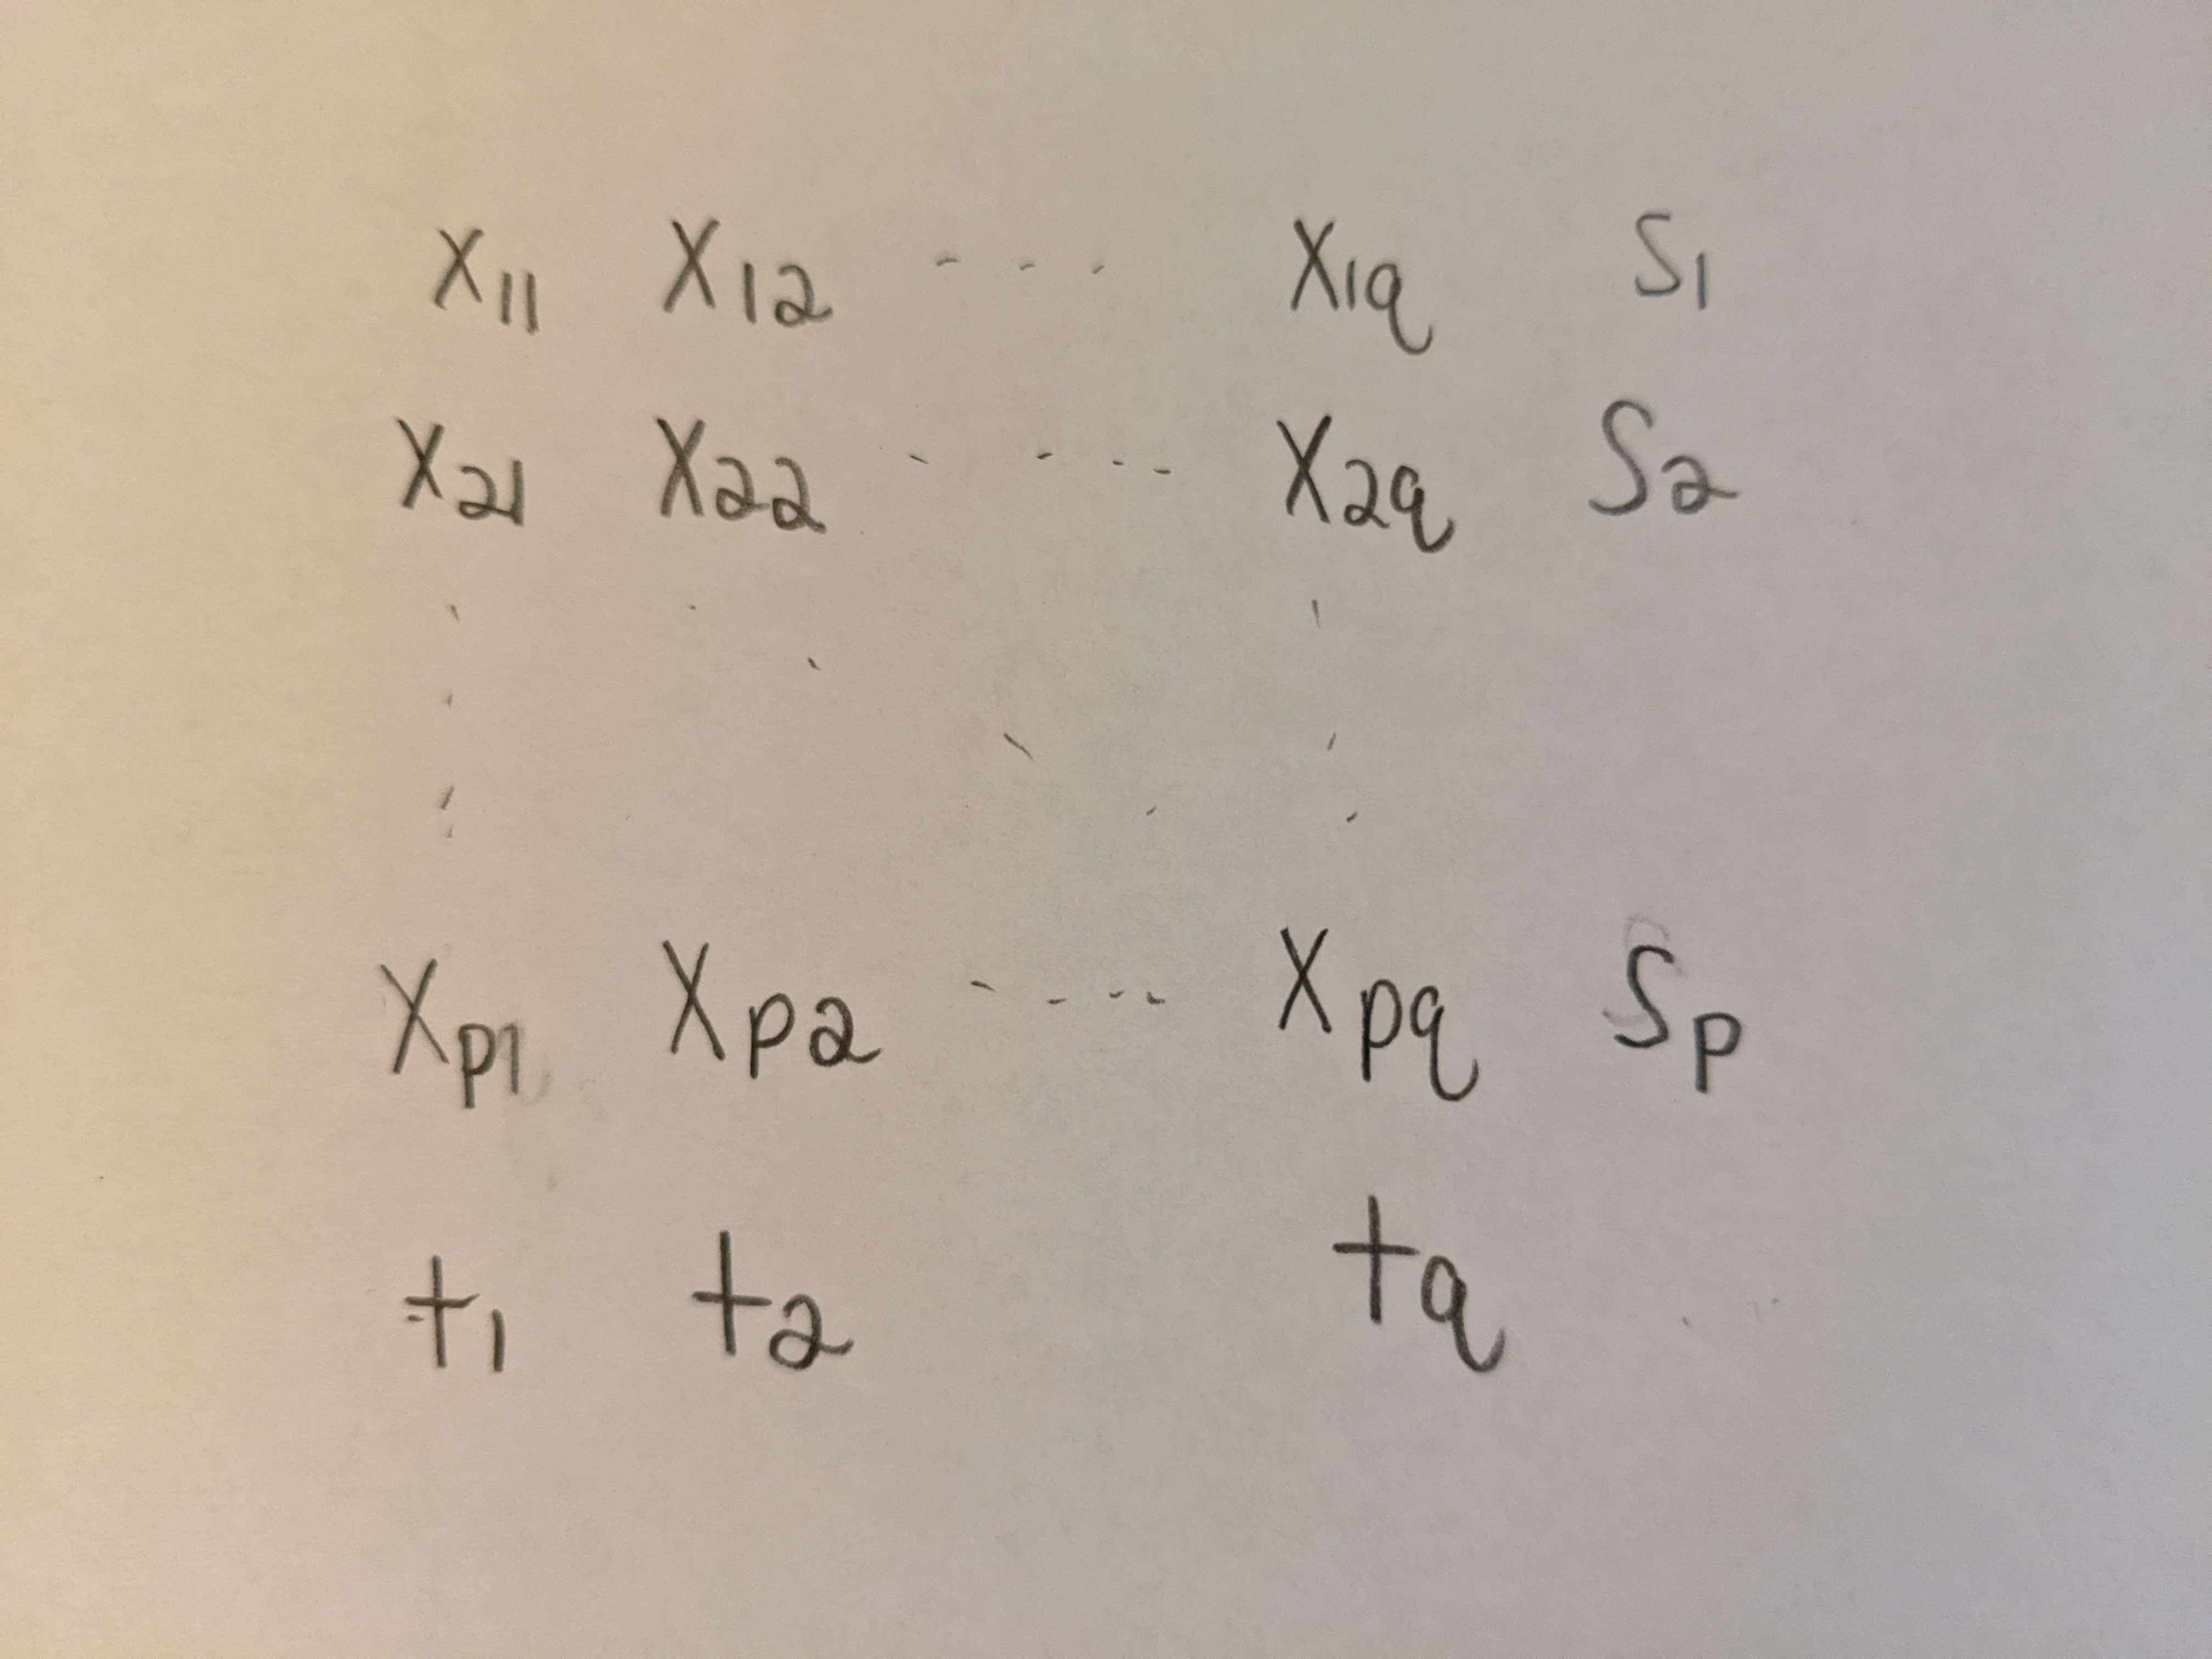
\includegraphics[width=\textwidth]{pic1}
%\end{figure}